\documentclass[11pt]{article}
\usepackage[margin=1in]{geometry}
\usepackage{amsmath,amssymb,amsthm}
\usepackage{algorithm}
\usepackage{algpseudocode}
\usepackage{booktabs}
\usepackage{hyperref}
\usepackage{xcolor}
\usepackage{tikz}
\usetikzlibrary{positioning,shapes.geometric,shapes.misc,arrows.meta,fit,backgrounds}

\newtheorem{definition}{Definition}
\newtheorem{theorem}{Theorem}
\newtheorem{proposition}{Proposition}
\newtheorem{example}{Example}

% --- Convenience macros (self-contained, mirror docs/macros.tex) -----------
\newcommand{\cK}{\mathcal{K}}
\newcommand{\cL}{\mathcal{L}}
\newcommand{\cG}{\mathcal{G}}
\newcommand{\cF}{\mathcal{F}}
\newcommand{\cS}{\mathcal{S}}
\newcommand{\cN}{\mathcal{N}}
\newcommand{\bp}{\mathbf{p}}
\newcommand{\bX}{\mathbf{X}}
\newcommand{\bY}{\mathbf{Y}}
\newcommand{\bZ}{\mathbf{Z}}
\newcommand{\bx}{\mathbf{x}}
\newcommand{\pa}{\mathrm{pa}}
\newcommand{\Pa}{\mathrm{Pa}}
\newcommand{\scc}{\mathrm{scc}}
\newcommand{\lo}{\underline}
\newcommand{\hi}{\overline}
\newcommand{\Vars}{\mathrm{Vars}}
\newcommand{\Iface}{\mathrm{Int}}      % interface variables
\newcommand{\fwd}{\mathrm{fwd}}
\newcommand{\bwd}{\mathrm{bwd}}

\title{SCC Factor-Graph Propagation\\
       A Hybrid Inference Algorithm for Logical Credal Networks}
\author{IBM Research}
\date{}

\begin{document}
\maketitle

\begin{abstract}
We describe \textbf{SCC Factor-Graph Propagation (SCC-FGP)}, a hybrid
approximate-inference algorithm for Logical Credal Networks (LCNs) that
computes lower/upper marginal probability bounds for all propositions.
The algorithm first decomposes the LCN's \emph{structure graph} into its
\textbf{Strongly Connected Components} (SCCs) using Tarjan's linear-time
algorithm, contracting every cycle into a single \emph{super-node}. The
result is a \emph{condensation graph}---a directed acyclic graph (DAG)---over
which we build a \textbf{factor graph} whose factor nodes are the super-nodes
and whose variable nodes are the \emph{interface variables} shared between
super-nodes. Belief propagation then runs \emph{exactly} on this acyclic
factor graph: messages are \emph{credal sets} (probability intervals on the
interface variables) and each factor-to-variable message is obtained by
solving a local non-linear program (NLP) over the joint space of one
super-node and its interface variables. Because all cycles are isolated
\emph{inside} the super-nodes, the global propagation is finite and exact
(two passes for a tree; one forward and one backward pass along a topological
order for a general DAG); the only source of approximation is the local NLP
solved inside a non-trivial (cyclic) super-node, which itself may be solved
exactly (e.g.\ \texttt{ipopt}) or approximately (e.g.\ ARIEL). We give the
full algorithm, complete pseudocode, and an end-to-end worked example on a
$7$-variable LCN ($A,B,C,D,E,X,Y$) with \emph{concrete numeric bounds} in which
we exhibit \emph{every} message, the exact NLP that produces it, and its
computed interval; the resulting marginals are verified to match the exact
$128$-world global NLP to four decimals. We close with a point-by-point
comparison against the ARIEL message-passing scheme, illustrated on the same
example.
\end{abstract}

\tableofcontents

%% =====================================================================
\section{Background: Logical Credal Networks}\label{sec:bg}
%% =====================================================================

A \textbf{Logical Credal Network} (LCN) is a probabilistic logic model that
combines propositional logic with imprecise (interval) probability bounds.
An LCN program $\cL$ is a finite set of labelled \textbf{sentences}, each of
one of two forms:
\begin{align}
  \text{(Type 1)}\quad & l \le P(\phi) \le u, \label{eq:type1}\\
  \text{(Type 2)}\quad & l \le P(\phi \mid \psi) \le u, \label{eq:type2}
\end{align}
where $\phi,\psi$ are propositional formulas over a set of Boolean atoms
(propositions) $\bX = \{X_1,\dots,X_n\}$ built from the connectives
\texttt{and}, \texttt{or}, \texttt{xor}, \texttt{nand}, \texttt{not}, and
$0\le l \le u \le 1$. Each sentence additionally carries a flag $\tau$ that
governs how it contributes to the structure graph (Section~\ref{sec:struct}).

\subsection{Semantics: the credal set}

An LCN does \emph{not} define a single joint distribution. Instead it defines
a \textbf{credal set} $\cK(\bX)$: the (convex) set of all joint probability
distributions $P$ over the $2^n$ truth assignments (``worlds'')
$\bx \in \{0,1\}^n$ that satisfy
\begin{enumerate}
  \item the \textbf{probability axioms}
        $\;p(\bx)\ge 0,\; \sum_{\bx} p(\bx) = 1$;
  \item every \textbf{probabilistic constraint} \eqref{eq:type1}--\eqref{eq:type2},
        where each probability is the sum of the world-probabilities consistent
        with the formula:
        \[
          P(\phi) = \sum_{\bx \,\models\, \phi} p(\bx), \qquad
          P(\phi\mid\psi) = \frac{P(\phi\wedge\psi)}{P(\psi)};
        \]
  \item the \textbf{Local Markov Condition (LMC)} independence constraints
        derived from the structure graph (below), each of which translates to a
        \emph{quadratic equality} of the form
        $P(\mathbf{x},\mathbf{y},\mathbf{z})\,P(\mathbf{z}) =
         P(\mathbf{x},\mathbf{z})\,P(\mathbf{y},\mathbf{z})$
        whenever $\bX\!\perp\!\bY \mid \bZ$.
\end{enumerate}
A Type-2 sentence $l \le P(\phi\mid\psi)\le u$ is \emph{linearized} into two
homogeneous linear inequalities over the world-probabilities,
\begin{equation}\label{eq:lin}
  l \cdot P(\psi) \;\le\; P(\phi\wedge\psi) \;\le\; u\cdot P(\psi),
\end{equation}
which become \emph{non-linear} only when $P(\psi)$ is itself an optimization
variable (a sum of $p(\bx)$). This is the sole source of non-convexity in the
feasible region.

\subsection{Marginal inference}

Given a query proposition $Q$, marginal inference computes the tightest bounds
\begin{equation}\label{eq:query}
  \lo P(Q) = \min_{P\in\cK(\bX)} \!\!\sum_{\bx\models Q}\!\! p(\bx),
  \qquad
  \hi P(Q) = \max_{P\in\cK(\bX)} \!\!\sum_{\bx\models Q}\!\! p(\bx).
\end{equation}
Solving \eqref{eq:query} over the full credal set is a single global NLP with
$2^n$ variables; it is exact but intractable (exponential variables,
non-convex) for all but the smallest LCNs. SCC-FGP is a \emph{structured}
approximation of this global problem.

\subsection{The structure graph}\label{sec:struct}

The structure graph $\cG_{\text{struct}}$ is a \emph{mixed} graph (directed
$+$ undirected edges) over the atoms, built from the sentences by the
following rules (implemented in \texttt{LCN.build\_structure\_graph}):
\begin{enumerate}
  \item \textbf{Undirected edges (intra-formula).} For each sentence with
        $\tau=\text{True}$, add an undirected edge between every pair of atoms
        occurring in the \emph{conditioned} formula $\phi$.
  \item \textbf{Directed edges (conditioning).} For each Type-2 sentence
        $P(\phi\mid\psi)$, add a directed edge $u\!\to\!v$ from every atom
        $u\in\psi$ to every atom $v\in\phi$.
  \item \textbf{Bidirected collapse.} If both $u\!\to\!v$ and $v\!\to\!u$ are
        present, replace them by a single undirected edge $u\!-\!v$.
  \item \textbf{Cleanup.} Remove formula-nodes and duplicate edges.
\end{enumerate}
Edges of $\cG_{\text{struct}}$ encode probabilistic dependence. A directed
cycle in $\cG_{\text{struct}}$ marks a set of mutually-dependent atoms that
\emph{cannot} be ordered acyclically---these are exactly the cycles that make
loopy propagation schemes (Section~\ref{sec:ariel}) inexact.

%% =====================================================================
\section{From Cycles to a DAG: SCC Decomposition}\label{sec:scc}
%% =====================================================================

\subsection{Strongly connected components}

\begin{definition}[SCC]
A \textbf{strongly connected component} of a directed graph $\cG$ is a maximal
set of vertices $S$ such that for every pair $u,v\in S$ there is a directed
path $u\!\leadsto\!v$ and a directed path $v\!\leadsto\!u$ in $\cG$. A vertex
with no cycle through it forms a trivial (singleton) SCC.
\end{definition}

To apply SCC analysis we first orient $\cG_{\text{struct}}$: an undirected
edge $u\!-\!v$ (which records a symmetric / cyclic dependence) is treated as
the pair of directed edges $u\!\to\!v$ and $v\!\to\!u$, so that any atoms
tied by undirected edges automatically land in the same SCC. (Equivalently,
\texttt{LCN.simplify\_structure\_graph} already contracts each undirected
clique into one meta-node; the SCC step then operates on the remaining
directed graph and merges any further directed cycles.)

\begin{proposition}[Tarjan]
The SCCs of a directed graph $\cG=(V,E)$ can be computed in $O(|V|+|E|)$ time,
and they can be emitted in reverse topological order of the condensation graph.
\end{proposition}

\subsection{The condensation graph}

\begin{definition}[Condensation / super-node]
Contracting each SCC $S_j$ to a single \textbf{super-node} and keeping one
edge $S_i\!\to\!S_j$ whenever $\cG_{\text{struct}}$ has an edge from some atom
in $S_i$ to some atom in $S_j$ (with $i\ne j$) yields the
\textbf{condensation graph} $\cG_{\scc}$. $\cG_{\scc}$ is always a
\emph{directed acyclic graph} (DAG): any cycle among super-nodes would
contradict the maximality of SCCs.
\end{definition}

We write $\Vars(S_j)$ for the atoms inside super-node $S_j$. A super-node is
\textbf{trivial} if $|\Vars(S_j)|=1$ and the atom has no self-cycle, and
\textbf{cyclic} (non-trivial) otherwise. The whole point of the
decomposition is captured by:

\begin{quote}
\emph{Every directed cycle of the original network lives entirely inside some
super-node. The graph \emph{between} super-nodes is acyclic.}
\end{quote}

\subsection{Interface variables}

\begin{definition}[Interface variable]
An atom $V$ is an \textbf{interface variable} of super-node $S_j$ if $V$
participates in an edge of $\cG_{\scc}$ incident to $S_j$, i.e.\ $V$ is the
\emph{tail} of a linking constraint $S_j\!\to\!S_c$ (an output interface
toward child $S_c$) or the \emph{head/parent} atom referenced by an incoming
linking constraint $S_p\!\to\!S_j$. Interface variables are the only atoms
whose beliefs are exchanged between super-nodes; the remaining atoms are
\textbf{internal} (hidden) to their super-node.
\end{definition}

%% =====================================================================
\section{The Condensation Factor Graph}\label{sec:fg}
%% =====================================================================

SCC-FGP runs belief propagation not on $\cG_{\scc}$ directly but on a
\textbf{factor graph} $\cF$ derived from it---a bipartite graph with two node
types:
\begin{itemize}
  \item \textbf{Factor nodes} $[\,S_j\,]$ (squares): one per super-node. The
        factor $[\,S_j\,]$ \emph{owns} (i) the internal probabilistic
        constraints of $S_j$, (ii) the LMC quadratic constraints local to
        $\Vars(S_j)$, and (iii) the \emph{linking constraints}
        $l\le P(\phi\mid\psi)\le u$ that connect $S_j$ to a neighbour.
  \item \textbf{Variable nodes} $(V)$ (circles): one per interface variable
        $V$. A variable node holds the current \emph{belief} (credal set /
        interval) about $V$.
\end{itemize}
Edges connect a factor $[\,S_j\,]$ to a variable $(V)$ iff $V$ is an interface
variable of $S_j$. Because $\cG_{\scc}$ is a DAG and each interface variable
links exactly the super-nodes that mention it, $\cF$ inherits an acyclic
(tree- or polytree-shaped) topology at the level of super-nodes.

\subsection{Messages are credal sets}

\begin{definition}[Message]
A \textbf{message} on edge $(V)\!-\![\,S_j\,]$ is a credal set over the single
interface variable $V$. For a Boolean $V$ this is simply an interval
$\cK(V) = [\,l_V,\,u_V\,]$ bounding $P(V{=}1)$ (with
$P(V{=}0)\in[1{-}u_V,\,1{-}l_V]$). In general it is the marginal credal set
$\cK(V)$, a convex polytope; for multi-state interfaces it is a vector of
per-state intervals (or a polytope given by linear inequalities, e.g.\ from
Fourier--Motzkin elimination).
\end{definition}

There are two message types, with the standard belief-propagation roles.

\paragraph{Variable-to-factor message $\mu(V\!\to\!F)$.}
The belief about $V$ assembled from \emph{every neighbour of $V$ except} $F$:
\begin{equation}\label{eq:v2f}
  \mu(V\!\to\!F) \;=\; \bigcap_{F'\in\cN(V)\setminus\{F\}} \mu(F'\!\to\!V).
\end{equation}
``$\cap$'' is credal-set \emph{intersection}; for intervals it is
\[
  \mu(V\!\to\!F) = \Bigl[\;\max_{F'} l_{F'\to V},\;\;
                          \min_{F'} u_{F'\to V}\;\Bigr].
\]
A leaf variable (one neighbour) sends a \emph{vacuous} message $[0,1]$ if it
has received nothing, or simply forwards its single incoming message.

\paragraph{Factor-to-variable message $\mu(F\!\to\!V)$.}
The core computation. Factor $F=[\,S_j\,]$ tells $V$ what its own constraints,
plus the messages from its \emph{other} interface variables, imply about $V$.
This requires solving a \textbf{local NLP} over the joint space of
$\Vars(S_j)$ together with the interface atoms of $S_j$:
\begin{equation}\label{eq:f2v}
\begin{aligned}
  \mu(F\!\to\!V):\quad
  \lo P(V) &= \min_{\bp}\; P(V{=}1), \qquad
  \hi P(V)  = \max_{\bp}\; P(V{=}1),\\
  \text{s.t.}\quad
  &\textstyle\sum_{\mathbf{w}} p(\mathbf{w}) = 1,\quad p(\mathbf{w})\ge 0,\\
  &\text{internal + LMC + linking constraints of } S_j,\\
  &\text{message constraints } \mu(V'\!\to\!F)
      \text{ for every other interface } V'\!\ne\!V .
\end{aligned}
\end{equation}
Here $\bp = \{p(\mathbf{w})\}$ ranges over the joint distribution of $S_j$'s
atoms and its interface atoms, and ``$V{=}1$'' is the union of worlds
$\mathbf{w}$ in which $V$ is true. Incoming interval messages
$\mu(V'\!\to\!F)=[l',u']$ enter as the two linear inequalities
$l'\le P(V'{=}1)\le u'$.

\paragraph{Why a ratio sometimes appears (LP vs.\ LFP).}
When the message target is a \emph{marginal} $P(V)$, both objective and
constraints are linear in $\bp$ \emph{except} for the conditional (linking /
internal) constraints, which after the linearization \eqref{eq:lin} are
homogeneous linear inequalities---so a marginal message is computed by an
\textbf{LP} when no internal LMC quadratics are active, and by an
\textbf{NLP} when they are. If instead one needs bounds on a \emph{conditional}
$P(Q\mid E)=P(Q,E)/P(E)$, the objective is a ratio of linear forms---a
\textbf{Linear-Fractional Program (LFP)}---which is solved by the
\textbf{Charnes--Cooper transformation} (substitute $t=1/P(E)$,
$y(\mathbf{w})=t\,p(\mathbf{w})$) into an equivalent LP.

\subsection{Final belief}

After messages have flowed both ways, the final marginal credal set of an
interface variable $V$ is the intersection of \emph{all} messages arriving at
its variable node:
\begin{equation}\label{eq:final-iface}
  \cK(V) = \bigcap_{F\in\cN(V)} \mu(F\!\to\!V)
         = \Bigl[\max_F l_{F\to V},\;\min_F u_{F\to V}\Bigr].
\end{equation}
For an \textbf{internal} atom $W$ (hidden inside $S_j$, never on an edge of
$\cF$), we run one final NLP on $[\,S_j\,]$ constrained by \emph{all} final
incoming messages and optimize $P(W{=}1)$:
\begin{equation}\label{eq:final-internal}
  \cK(W) = \Bigl[\;\min_{\bp}P(W{=}1),\;\max_{\bp}P(W{=}1)\;\Bigr]
  \;\text{s.t. internal/LMC/linking constraints} +\!\!\!
  \bigcup_{V\in\Iface(S_j)}\!\!\!\mu(V\!\to\!F).
\end{equation}

%% =====================================================================
\section{The SCC-FGP Algorithm}\label{sec:alg}
%% =====================================================================

\subsection{Overview}
The algorithm has four stages:
\begin{enumerate}
  \item \textbf{Decompose.} Build $\cG_{\text{struct}}$, run Tarjan to get
        SCCs, contract into the condensation DAG $\cG_{\scc}$, identify
        interface variables, and build the factor graph $\cF$.
  \item \textbf{Collect (forward).} Process factors in a topological order;
        each factor, having received messages from its already-processed
        neighbours, emits factor-to-variable messages toward its children.
  \item \textbf{Distribute (backward).} Process factors in reverse topological
        order; each factor emits factor-to-variable messages back toward its
        parents.
  \item \textbf{Extract.} Compute final beliefs: intersect messages at each
        interface variable~\eqref{eq:final-iface}; solve one local NLP per
        super-node for its internal atoms~\eqref{eq:final-internal}.
\end{enumerate}
For a \emph{tree}-shaped factor graph this is exactly two passes
(collect-to-root, distribute-from-root). For a general DAG of super-nodes the
forward pass follows a topological sort and the backward pass its reverse;
each factor combines \emph{all} incoming messages from already-processed
neighbours before emitting, which is the generalized (non-loopy) belief
propagation rule.

\subsection{Pseudocode}

\begin{algorithm}[H]
\caption{SCC Factor-Graph Propagation (SCC-FGP)}
\label{alg:sccfgp}
\begin{algorithmic}[1]
\Require LCN $\cL$; local-solver \textsc{Solve} (exact \texttt{ipopt} or ARIEL)
\Ensure Bounds $[\lo P(W),\hi P(W)]$ for every atom $W$
\Statex
\Comment{\textsc{Stage 1 --- Decompose}}
\State $\cG_{\text{struct}} \gets \textsc{BuildStructureGraph}(\cL)$
\State Orient undirected edges as symmetric directed pairs
\State $\{S_1,\dots,S_k\} \gets \textsc{Tarjan}(\cG_{\text{struct}})$
       \Comment{SCCs, $O(|V|{+}|E|)$}
\State $\cG_{\scc} \gets \textsc{Condense}(\cG_{\text{struct}},\{S_j\})$
       \Comment{DAG of super-nodes}
\State Identify interface variables; build factor graph $\cF$
\State $\mathbf{o} \gets \textsc{TopologicalSort}(\cG_{\scc})$
\Statex
\Comment{\textsc{Stage 2 --- Collect (forward, order $\mathbf{o}$)}}
\For{each factor $[S_i]$ in order $\mathbf{o}$}
  \State Gather incoming $\mu(V\!\to\![S_i])$ from already-processed
         neighbours \Comment{Eq.~\eqref{eq:v2f}}
  \For{each child interface $V$ of $[S_i]$}
     \State $\mu(S_i\!\to\!V) \gets \textsc{Solve}\bigl(\text{local NLP
            \eqref{eq:f2v} for } V\bigr)$
     \State Push $\mu(S_i\!\to\!V)$ onto variable node $(V)$
  \EndFor
\EndFor
\Statex
\Comment{\textsc{Stage 3 --- Distribute (backward, order reverse $\mathbf{o}$)}}
\For{each factor $[S_i]$ in reverse order $\mathbf{o}$}
  \State Gather incoming $\mu(V\!\to\![S_i])$ from all neighbours
         except the target \Comment{Eq.~\eqref{eq:v2f}}
  \For{each parent interface $V$ of $[S_i]$}
     \State $\mu(S_i\!\to\!V) \gets \textsc{Solve}\bigl(\text{local NLP
            \eqref{eq:f2v} for } V\bigr)$
     \State Push $\mu(S_i\!\to\!V)$ onto variable node $(V)$
  \EndFor
\EndFor
\Statex
\Comment{\textsc{Stage 4 --- Extract marginals}}
\For{each interface variable $V$}
  \State $\cK(V)\gets\bigl[\max_F l_{F\to V},\ \min_F u_{F\to V}\bigr]$
         \Comment{Eq.~\eqref{eq:final-iface}}
\EndFor
\For{each super-node $S_j$}
  \For{each internal atom $W\in\Vars(S_j)$}
     \State $\cK(W)\gets\textsc{Solve}\bigl(\text{final NLP
            \eqref{eq:final-internal} for }W\bigr)$
  \EndFor
\EndFor
\State \Return $\{[\lo P(W),\hi P(W)]\}_{W\in\bX}$
\end{algorithmic}
\end{algorithm}

\begin{theorem}[Finiteness and global exactness]
On the acyclic factor graph $\cF$, SCC-FGP terminates after exactly one
forward and one backward pass over the $k$ super-nodes, computing
$O(|E(\cF)|)$ messages. If every local NLP \eqref{eq:f2v} is solved to global
optimality, the propagation introduces \emph{no} additional looseness beyond
the structured (per-super-node marginalization) approximation: there is no
double-counting of evidence, because no message ever traverses a cycle at the
super-node level.
\end{theorem}

\begin{proposition}[Sole source of approximation]
The only approximation in SCC-FGP arises \emph{inside} a cyclic super-node
whose local NLP \eqref{eq:f2v} is too large to solve exactly and is instead
handed to an approximate solver (e.g.\ ARIEL). Trivial (acyclic) super-nodes
yield LPs/LFPs solved exactly.
\end{proposition}

%% =====================================================================
\section{Worked Example: a 7-Variable LCN}\label{sec:example}
%% =====================================================================

We now make every step concrete on a $7$-proposition LCN whose condensation
graph is a non-trivial (non-tree) DAG, so that the general multi-parent /
multi-child message rules are exercised.

\subsection{The LCN}

\paragraph{Propositions (7):} $\{X,\,Y,\,A,\,B,\,C,\,D,\,E\}$.

\paragraph{Constraints (with concrete numeric bounds):}
\begin{center}
\begin{tabular}{llll}
\toprule
Label & Sentence & Numeric form & Role \\
\midrule
$c_X$    & $P(X)$        & $\in[0.60,\,0.80]$ & root prior \\
$c_Y$    & $P(Y)$        & $\in[0.30,\,0.50]$ & root prior \\
$c_{XA}$ & $P(A\mid X)$  & $\in[0.70,\,0.90]$ & link $X\!\to\!A$ \\
$c_{YB}$ & $P(B\mid Y)$  & $\in[0.20,\,0.40]$ & link $Y\!\to\!B$ \\
$c_{AB}$ & $P(B\mid A)$  & $\in[0.50,\,0.70]$ & link $A\!\to\!B$ \\
$c_{BC}$ & $P(C\mid B)$  & $\in[0.60,\,0.80]$ & \emph{cycle} edge \\
$c_{CD}$ & $P(D\mid C)$  & $\in[0.40,\,0.60]$ & \emph{cycle} edge \\
$c_{DB}$ & $P(B\mid D)$  & $\in[0.30,\,0.50]$ & \emph{cycle} edge \\
$c_{CE}$ & $P(E\mid C)$  & $\in[0.80,\,0.90]$ & link $C\!\to\!E$ \\
$c_{\bar C E}$ & $P(E\mid \neg C)$ & $\in[0.10,\,0.30]$ & link $C\!\to\!E$ \\
$c_E$    & $P(E)$        & $\in[0.50,\,0.70]$ & leaf prior \\
\bottomrule
\end{tabular}
\end{center}

\noindent The last two sentences, $c_{\bar C E}$ and $c_E$, are added so that the
\emph{backward} pass carries real information: $c_E$ pins the marginal of the
leaf $E$, and together with $c_{CE},c_{\bar C E}$ this constrains $P(C)$ when
propagated back up. (Without them, every backward message in this all-``downward''
network would be the vacuous interval $[0,1]$.)

\paragraph{LCN conditional semantics.}
A Type-2 sentence $l\le P(H\mid G)\le u$ constrains \emph{only} the conditioning
event $G{=}\text{true}$; via \eqref{eq:lin} it becomes the single pair of
inequalities $l\,P(G{=}1)\le P(H{=}1,G{=}1)\le u\,P(G{=}1)$. (The reverse case
$G{=}\text{false}$ is governed by a \emph{separate} sentence, e.g.\ $c_{\bar C E}$
covers $E\mid\neg C$.) This matches the encoding in
\texttt{lcn/inference/marginal/exact.py}.

\paragraph{Structure graph.}
The directed edges are
$X\!\to\!A,\;Y\!\to\!B,\;A\!\to\!B,\;B\!\to\!C,\;C\!\to\!D,\;D\!\to\!B,\;C\!\to\!E$
(the formula $\neg C$ in $c_{\bar C E}$ contributes the same edge $C\!\to\!E$).
The three constraints $c_{BC},c_{CD},c_{DB}$ form a directed cycle
$B\!\to\!C\!\to\!D\!\to\!B$.

\subsection{SCC decomposition}

Tarjan's algorithm finds one non-trivial SCC,
$S_{BCD}=\{B,C,D\}$ (the cycle), and four trivial SCCs
$S_X=\{X\},\,S_Y=\{Y\},\,S_A=\{A\},\,S_E=\{E\}$. The condensation graph
$\cG_{\scc}$ is the DAG
\[
  S_X \to S_A \to S_{BCD},\qquad
  S_Y \to S_{BCD},\qquad
  S_{BCD}\to S_E .
\]
A valid topological order is $\mathbf{o}=(S_X,\,S_Y,\,S_A,\,S_{BCD},\,S_E)$.
The \textbf{interface variables} are $X$ (links $S_X\!-\!S_A$), $A$ (links
$S_A\!-\!S_{BCD}$), $Y$ (links $S_Y\!-\!S_{BCD}$), $C$ (links
$S_{BCD}\!-\!S_E$), and $E$ (output of $S_E$). The atoms $B$ and $D$ are
\textbf{internal} to $S_{BCD}$.

\subsection{The condensation factor graph}

\begin{center}
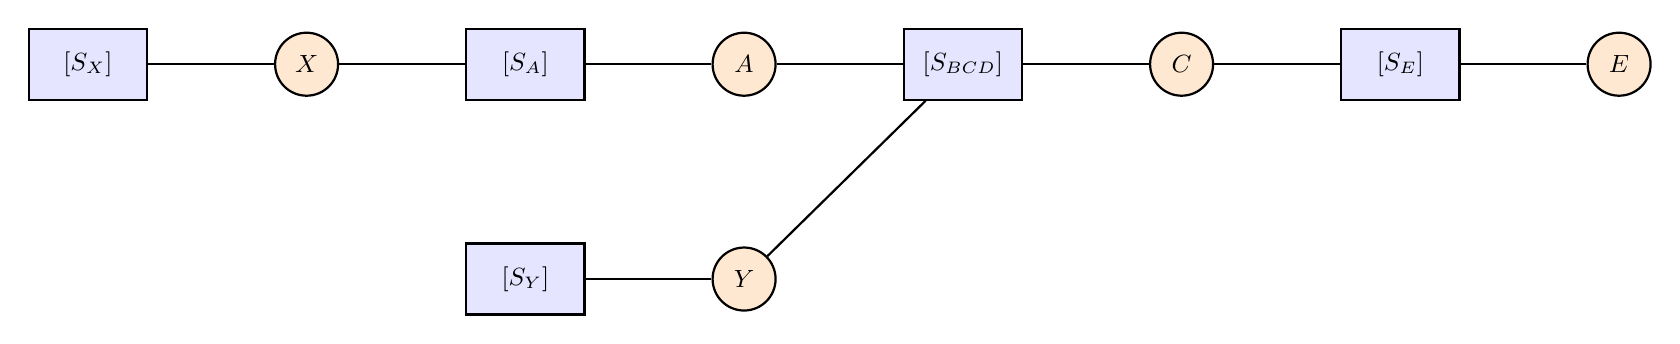
\begin{tikzpicture}[
  fac/.style={rectangle, draw, thick, minimum width=15mm, minimum height=9mm,
              font=\small, fill=blue!10},
  var/.style={circle, draw, thick, minimum size=8mm, font=\small,
              fill=orange!18},
  e/.style={thick},
  node distance=14mm and 16mm
]
  % factor nodes
  \node[fac] (SX)  {$[S_X]$};
  \node[var, right=of SX] (X) {$X$};
  \node[fac, right=of X]  (SA) {$[S_A]$};
  \node[var, right=of SA] (A) {$A$};
  \node[fac, right=of A]  (SBCD) {$[S_{BCD}]$};
  \node[var, right=of SBCD] (C) {$C$};
  \node[fac, right=of C]  (SE) {$[S_E]$};
  \node[var, right=of SE] (E) {$E$};
  % Y branch below
  \node[fac, below=18mm of SA] (SY) {$[S_Y]$};
  \node[var, right=of SY] (Y) {$Y$};

  \draw[e] (SX)--(X); \draw[e] (X)--(SA); \draw[e] (SA)--(A);
  \draw[e] (A)--(SBCD); \draw[e] (SBCD)--(C); \draw[e] (C)--(SE);
  \draw[e] (SE)--(E);
  \draw[e] (SY)--(Y); \draw[e] (Y)-- (SBCD);
\end{tikzpicture}
\end{center}

Squares are factor nodes (super-nodes), circles are interface variable nodes.
Edges: $(X)\!-\![S_X],[S_A]$; $(A)\!-\![S_A],[S_{BCD}]$;
$(Y)\!-\![S_Y],[S_{BCD}]$; $(C)\!-\![S_{BCD}],[S_E]$; $(E)\!-\![S_E]$. The
factor graph is a \textbf{tree} with hub $[S_{BCD}]$; we root it at $[S_E]$
and run two passes.

\medskip
\noindent\emph{Notation for the worked NLPs.} Inside a factor we index joint
probabilities by the truth values of the relevant atoms; e.g.\ in $[S_A]$,
$p_{ax}=P(A{=}a,X{=}x)$; in $[S_E]$, $p_{ec}=P(E{=}e,C{=}c)$; in $[S_{BCD}]$,
$p_{bcday}=P(B{=}b,C{=}c,D{=}d,A{=}a,Y{=}y)$ ($2^5=32$ variables). A linking
constraint such as $c_{AB}: 0.50\le P(B\mid A)\le 0.70$ expands (via
\eqref{eq:lin}, for the conditioning event $A{=}1$ \emph{only}) to the single
pair
$0.50\,P(A{=}1)\le P(B{=}1,A{=}1)\le 0.70\,P(A{=}1)$, each side a sum of the
$p$-variables. There is \emph{no} companion constraint for $A{=}0$ unless a
separate sentence (such as $c_{\bar C E}$ for $E\mid\neg C$) supplies one.

\medskip
\noindent\emph{All intervals below are the actual optimal values} produced by
solving the stated LP/NLP for the numeric bounds of the constraint table. As a
ground-truth check, the single global NLP over all $2^7=128$ worlds
(Section~\ref{sec:bg}) yields \emph{identical} final marginals
(Section~\ref{sec:final}, Table~\ref{tab:final}): on this network the
condensation graph is a polytree and every SCC is solved exactly, so SCC-FGP is
\emph{exact} here.

%% --------------------------------------------------------------
\subsection{Pass 1 --- Collect (toward root $[S_E]$)}
%% --------------------------------------------------------------

\paragraph{(1.1) $\mu(S_X\!\to\!X)$ --- LP.}
\begin{align*}
  \text{Variable: } & p_x = P(X{=}1).\\
  \text{Constraints: } & 0.60 \le p_x \le 0.80. \\
  \text{Objective: } & \min/\max\; p_x .\\
  \Rightarrow\;& \mu(S_X\!\to\!X)=\cK(X)=[\,0.60,\,0.80\,].
\end{align*}

\paragraph{(1.2) $\mu(S_Y\!\to\!Y)$ --- LP.}
Symmetric: variable $p_y$, constraint $0.30\le p_y\le 0.50$,
$\Rightarrow \mu(S_Y\!\to\!Y)=\cK(Y)=[\,0.30,\,0.50\,].$

\paragraph{(1.3) $\mu(X\!\to\!S_A)$ and $\mu(Y\!\to\!S_{BCD})$ --- V$\to$F.}
$(X)$ has one other neighbour, so it forwards its incoming message:
$\mu(X\!\to\!S_A)=[\,0.60,0.80\,]$. Likewise
$\mu(Y\!\to\!S_{BCD})=[\,0.30,0.50\,]$.

\paragraph{(1.4) $\mu(S_A\!\to\!A)$ --- NLP over $\{A,X\}$.}
\begin{align*}
  \text{Variables: } & p_{ax},\ a,x\in\{0,1\}\quad(4\text{ vars}).\\
  \text{Constraints: } & \textstyle\sum_{ax}p_{ax}=1,\quad p_{ax}\ge0;\\
                       & \text{incoming } \mu(X\!\to\!S_A):\ 0.60\le (p_{01}{+}p_{11})\le 0.80;\\
                       & c_{XA}\ (X{=}1\text{ only}):\
                          0.70\,(p_{01}{+}p_{11})\le p_{11}\le 0.90\,(p_{01}{+}p_{11}).\\
  \text{Objective: } & \min/\max\; P(A{=}1)=p_{10}{+}p_{11}.\\
  \Rightarrow\;& \mu(S_A\!\to\!A)=\cK_\fwd(A)=[\,0.4200,\,0.9400\,].
\end{align*}
(\emph{Why so wide?} $c_{XA}$ pins $A$ only through $X{=}1$; the mass on
$X{=}0$ leaves $P(A{=}1\mid X{=}0)$ unconstrained, so the lower bound
$0.70\!\cdot\!0.60=0.42$ and upper bound $0.90\!\cdot\!0.60+0.40=0.94$ follow.)

\paragraph{(1.5) $\mu(A\!\to\!S_{BCD})$ --- V$\to$F.}
$(A)$ forwards: $\mu(A\!\to\!S_{BCD})=\cK_\fwd(A)=[\,0.4200,0.9400\,]$.

\paragraph{(1.6) $\mu(S_{BCD}\!\to\!C)$ --- the large NLP over $\{B,C,D,A,Y\}$.}
This is the heart of the example: it isolates the cycle. Every conditional
below is enforced for its conditioning event $={}$true \emph{only}.
\begin{align*}
  \text{Variables: } & p_{bcday},\ b,c,d,a,y\in\{0,1\}\quad(32\text{ vars}).\\
  \text{Constraints: } & \textstyle\sum p_{bcday}=1,\quad p_{bcday}\ge0;\\
   \text{(incoming)}\;& 0.4200 \le P(A{=}1)=\!\!\sum_{b,c,d,y}\!\!p_{bcd1y} \le 0.9400; \\
                      & 0.30 \le P(Y{=}1)=\!\!\sum_{b,c,d,a}\!\!p_{bcda1} \le 0.50; \\
   \text{(linking)}\;& c_{AB}:\ 0.50\,P(A{=}1)\!\le\! P(B{=}1,A{=}1)\!\le\! 0.70\,P(A{=}1);\\
                      & c_{YB}:\ 0.20\,P(Y{=}1)\!\le\! P(B{=}1,Y{=}1)\!\le\! 0.40\,P(Y{=}1);\\
   \text{(internal,}&\text{ cyclic)}\quad
                      c_{BC}:\ 0.60\,P(B{=}1)\le P(C{=}1,B{=}1)\le 0.80\,P(B{=}1);\\
                      & c_{CD}:\ 0.40\,P(C{=}1)\le P(D{=}1,C{=}1)\le 0.60\,P(C{=}1);\\
                      & c_{DB}:\ 0.30\,P(D{=}1)\le P(B{=}1,D{=}1)\le 0.50\,P(D{=}1).\\
  \text{Objective: } & \min/\max\; P(C{=}1)=\!\!\sum_{a,b,d,y}\!\!p_{b1day}.\\
  \Rightarrow\;& \mu(S_{BCD}\!\to\!C)=\cK_\fwd(C)=[\,0.1260,\,0.9580\,].
\end{align*}
The three constraints $c_{BC},c_{CD},c_{DB}$ are mutually dependent (the
cycle); solving this NLP \emph{jointly} over all $32$ worlds is precisely what
captures the cyclic dependence exactly, instead of looping messages around it.

\paragraph{(1.7) $\mu(C\!\to\!S_E)$ --- V$\to$F.}
$(C)$ forwards: $\mu(C\!\to\!S_E)=\cK_\fwd(C)=[\,0.1260,0.9580\,]$. The
root factor $[S_E]$ has now received all leaf-ward information.

%% --------------------------------------------------------------
\subsection{Pass 2 --- Distribute (away from root $[S_E]$)}
%% --------------------------------------------------------------

\paragraph{(2.1) $\mu(S_E\!\to\!C)$ --- NLP over $\{E,C\}$.}
Per the BP rule, the backward message out of $[S_E]$ to $(C)$ uses $[S_E]$'s
\emph{other} inputs only and therefore \emph{excludes} the message
$\mu(C\!\to\!S_E)$ that just arrived from $C$. What remains are $[S_E]$'s own
constraints $c_{CE}$ ($E\mid C$), $c_{\bar C E}$ ($E\mid\neg C$) and the leaf
prior $c_E$ ($P(E)$). It is precisely $c_E$ together with the two-sided
$c_{CE},c_{\bar C E}$ that lets $E$ ``speak back'' about $C$.
\begin{align*}
  \text{Variables: } & p_{ec},\ e,c\in\{0,1\}\quad(4\text{ vars}).\\
  \text{Constraints: } & \textstyle\sum_{ec}p_{ec}=1,\quad p_{ec}\ge0;\\
                       & c_{CE}\ (C{=}1):\ 0.80\,(p_{01}{+}p_{11})\le p_{11}\le 0.90\,(p_{01}{+}p_{11});\\
                       & c_{\bar C E}\ (C{=}0):\ 0.10\,(p_{00}{+}p_{10})\le p_{10}\le 0.30\,(p_{00}{+}p_{10});\\
                       & c_E:\ 0.50 \le P(E{=}1)=p_{10}{+}p_{11}\le 0.70.\\
  \text{Objective: } & \min/\max\; P(C{=}1)=p_{01}{+}p_{11}.\\
  \Rightarrow\;& \mu(S_E\!\to\!C)=\cK_\bwd(C)=[\,0.3333,\,0.8571\,].
\end{align*}
Intuition: $P(E)=P(E\mid C)P(C)+P(E\mid\neg C)P(\neg C)$ with $P(E)\le 0.70$
and $P(E\mid C)\ge 0.80$ forces $P(C)\le 0.857$; with $P(E)\ge 0.50$ and
$P(E\mid\neg C)\le 0.30$ it forces $P(C)\ge 0.333$.

\paragraph{(2.2) $\mu(C\!\to\!S_{BCD})$ --- V$\to$F.}
$\mu(C\!\to\!S_{BCD})=\cK_\bwd(C)=[\,0.3333,0.8571\,]$.

\paragraph{(2.3) $\mu(S_{BCD}\!\to\!A)$ --- large NLP, objective on $A$.}
Same $32$-variable factor, but now the incoming messages are
$\mu(Y\!\to\!S_{BCD})=[\,0.30,0.50\,]$ (forward) and
$\mu(C\!\to\!S_{BCD})=[\,0.3333,0.8571\,]$ (backward); the message from
$A$ is \emph{excluded}.
\begin{align*}
  \text{Constraints: } & \textstyle\sum p_{bcday}=1,\ p\ge0;\quad
                          0.30\le P(Y{=}1)\le 0.50;\\
                       & 0.3333\le P(C{=}1)\le 0.8571;\\
                       & \text{linking } c_{YB}\text{; internal } c_{BC},c_{CD},c_{DB}\ (\text{cond.\ true only}).\\
  \text{Objective: } & \min/\max\; P(A{=}1)=\!\!\sum_{b,c,d,y}\!\!p_{bcd1y}.\\
  \Rightarrow\;& \mu(S_{BCD}\!\to\!A)=\cK_\bwd(A)=[\,0.0000,\,1.0000\,].
\end{align*}
The result is \emph{vacuous}: the only constraint touching $A$ is $c_{AB}$
($B\mid A$), which is excluded here (it lives on the $A$ edge), and the
internal constraints constrain $B,C,D$ but impose no \emph{lower} or
\emph{upper} bound back onto the marginal $P(A)$ given the available messages.
Information in this network flows strictly downstream, so the backward message
to a parent carries nothing.

\paragraph{(2.4) $\mu(S_{BCD}\!\to\!Y)$ --- large NLP, objective on $Y$.}
Symmetric to (2.3): incoming $\mu(A\!\to\!S_{BCD})=[\,0.4200,0.9400\,]$
(forward) and $\mu(C\!\to\!S_{BCD})=[\,0.3333,0.8571\,]$ (backward), exclude
$Y$; linking $c_{AB}$; internal $c_{BC},c_{CD},c_{DB}$; objective
$\min/\max P(Y{=}1)$ (through the excluded $c_{YB}$). $\Rightarrow
\mu(S_{BCD}\!\to\!Y)=\cK_\bwd(Y)=[\,0.0000,1.0000\,]$ --- again vacuous, for the
same reason.

\paragraph{(2.5) $\mu(A\!\to\!S_A)$ --- V$\to$F.}
$\mu(A\!\to\!S_A)=\cK_\bwd(A)=[\,0.0000,1.0000\,]$.

\paragraph{(2.6) $\mu(S_A\!\to\!X)$ --- NLP over $\{A,X\}$.}
\begin{align*}
  \text{Variables: } & p_{ax}\ (4\text{ vars}).\\
  \text{Constraints: } & \textstyle\sum p_{ax}=1,\ p\ge0;\quad
                          \mu(A\!\to\!S_A){:}\ 0.0\le P(A{=}1)=(p_{10}{+}p_{11})\le 1.0;\\
                       & c_{XA}\ (X{=}1\text{ only}).\\
  \text{Objective: } & \min/\max\; P(X{=}1)=p_{01}{+}p_{11}.\\
  \Rightarrow\;& \mu(S_A\!\to\!X)=\cK_\bwd(X)=[\,0.0000,\,1.0000\,].
\end{align*}
Vacuous, because the incoming backward message on $A$ is itself vacuous and
$c_{XA}$ constrains $A\mid X$, not $X$.

\paragraph{(2.7) $\mu(Y\!\to\!S_Y)$ --- V$\to$F.}
$\mu(Y\!\to\!S_Y)=\cK_\bwd(Y)=[\,0.0000,1.0000\,]$ (used only if a final
belief at $Y$ is desired; $[S_Y]$ has no further constraints to add).

%% --------------------------------------------------------------
\subsection{Stage 4 --- Final marginals}
%% --------------------------------------------------------------

\label{sec:final}
\paragraph{Interface variables (intersection, Eq.~\eqref{eq:final-iface}).}
\begin{align*}
  \cK(X) &= \mu(S_X\!\to\!X)\cap\mu(S_A\!\to\!X)
          = [0.60,0.80]\cap[0,1] = [\,0.6000,\,0.8000\,],\\
  \cK(A) &= \mu(S_A\!\to\!A)\cap\mu(S_{BCD}\!\to\!A)
          = [0.42,0.94]\cap[0,1] = [\,0.4200,\,0.9400\,],\\
  \cK(Y) &= \mu(S_Y\!\to\!Y)\cap\mu(S_{BCD}\!\to\!Y)
          = [0.30,0.50]\cap[0,1] = [\,0.3000,\,0.5000\,],\\
  \cK(C) &= \mu(S_{BCD}\!\to\!C)\cap\mu(S_E\!\to\!C)
          = [0.126,0.958]\cap[0.333,0.857] = [\,0.3333,\,0.8571\,],\\
  \cK(E) &= \mu(S_E\!\to\!E)= [\,0.5000,\,0.7000\,]\quad(\text{one NLP on }[S_E]\text{ with }c_{CE},c_{\bar C E},c_E).
\end{align*}
Only $\cK(C)$ is tightened by the backward pass (the two messages genuinely
intersect, $0.333=\max(0.126,0.333)$ and $0.857=\min(0.958,0.857)$); the other
interfaces inherit their forward intervals because every backward message was
vacuous.

\paragraph{Internal atoms $B,D$ (Eq.~\eqref{eq:final-internal}).}
Run one last NLP on $[S_{BCD}]$ ($32$ vars) constrained by \emph{all} final
incoming messages $\mu(A\!\to\!S_{BCD})=[0.42,0.94]$,
$\mu(Y\!\to\!S_{BCD})=[0.30,0.50]$, $\mu(C\!\to\!S_{BCD})=[0.3333,0.8571]$, plus
internal $c_{BC},c_{CD},c_{DB}$ and linking $c_{AB},c_{YB}$; objectives
$\min/\max P(B{=}1)$ and $\min/\max P(D{=}1)$:
\[
  \cK(B)=[\,0.2100,\,0.8200\,],\qquad \cK(D)=[\,0.1333,\,0.8667\,].
\]

\paragraph{Final marginals and exactness check.}
Table~\ref{tab:final} lists the SCC-FGP marginals beside the bounds from the
single global NLP over all $2^7=128$ worlds (Section~\ref{sec:bg}). They are
\emph{identical} to four decimals: on this network the condensation graph is a
polytree and every super-node NLP is solved exactly, so SCC-FGP attains the
true tightest bounds.

\begin{table}[h]
\centering
\caption{SCC-FGP marginals vs.\ the exact global NLP (all $128$ worlds).}
\label{tab:final}
\begin{tabular}{lcc c}
\toprule
Variable & SCC-FGP $[\lo P,\hi P]$ & Global (exact) & Match \\
\midrule
$A$ & $[0.4200,\,0.9400]$ & $[0.4200,\,0.9400]$ & \checkmark \\
$B$ & $[0.2100,\,0.8200]$ & $[0.2100,\,0.8200]$ & \checkmark \\
$C$ & $[0.3333,\,0.8571]$ & $[0.3333,\,0.8571]$ & \checkmark \\
$D$ & $[0.1333,\,0.8667]$ & $[0.1333,\,0.8667]$ & \checkmark \\
$E$ & $[0.5000,\,0.7000]$ & $[0.5000,\,0.7000]$ & \checkmark \\
$X$ & $[0.6000,\,0.8000]$ & $[0.6000,\,0.8000]$ & \checkmark \\
$Y$ & $[0.3000,\,0.5000]$ & $[0.3000,\,0.5000]$ & \checkmark \\
\bottomrule
\end{tabular}
\end{table}

\subsection{Summary of all messages}

\begin{center}
\begin{tabular}{lllcl}
\toprule
\textbf{Pass} & \textbf{Message} & \textbf{Type} & \textbf{NLP vars} & \textbf{Result interval} \\
\midrule
collect & $\mu(S_X\!\to\!X)$        & F$\to$V (LP)  & 1  & $[0.6000,\,0.8000]$ \\
collect & $\mu(S_Y\!\to\!Y)$        & F$\to$V (LP)  & 1  & $[0.3000,\,0.5000]$ \\
collect & $\mu(X\!\to\!S_A)$        & V$\to$F       & -- & $[0.6000,\,0.8000]$ \\
collect & $\mu(Y\!\to\!S_{BCD})$    & V$\to$F       & -- & $[0.3000,\,0.5000]$ \\
collect & $\mu(S_A\!\to\!A)$        & F$\to$V (NLP) & 4  & $[0.4200,\,0.9400]$ \\
collect & $\mu(A\!\to\!S_{BCD})$    & V$\to$F       & -- & $[0.4200,\,0.9400]$ \\
collect & $\mu(S_{BCD}\!\to\!C)$    & F$\to$V (NLP) & 32 & $[0.1260,\,0.9580]$ \\
collect & $\mu(C\!\to\!S_E)$        & V$\to$F       & -- & $[0.1260,\,0.9580]$ \\
\midrule
distribute & $\mu(S_E\!\to\!C)$     & F$\to$V (NLP) & 4  & $[0.3333,\,0.8571]$ \\
distribute & $\mu(C\!\to\!S_{BCD})$ & V$\to$F       & -- & $[0.3333,\,0.8571]$ \\
distribute & $\mu(S_{BCD}\!\to\!A)$ & F$\to$V (NLP) & 32 & $[0.0000,\,1.0000]$ (vac.) \\
distribute & $\mu(S_{BCD}\!\to\!Y)$ & F$\to$V (NLP) & 32 & $[0.0000,\,1.0000]$ (vac.) \\
distribute & $\mu(A\!\to\!S_A)$     & V$\to$F       & -- & $[0.0000,\,1.0000]$ (vac.) \\
distribute & $\mu(S_A\!\to\!X)$     & F$\to$V (NLP) & 4  & $[0.0000,\,1.0000]$ (vac.) \\
distribute & $\mu(Y\!\to\!S_Y)$     & V$\to$F       & -- & $[0.0000,\,1.0000]$ (vac.) \\
\midrule
extract & $\cK(X)$                  & intersect & -- & $[0.6000,\,0.8000]$ \\
extract & $\cK(A)$                  & intersect & -- & $[0.4200,\,0.9400]$ \\
extract & $\cK(Y)$                  & intersect & -- & $[0.3000,\,0.5000]$ \\
extract & $\cK(C)$                  & intersect & -- & $[0.3333,\,0.8571]$ \\
extract & $\cK(B),\cK(D)$           & F final (NLP) & 32 & $[0.2100,0.8200],[0.1333,0.8667]$ \\
extract & $\cK(E)$                  & F final (NLP) & 4  & $[0.5000,\,0.7000]$ \\
\bottomrule
\end{tabular}
\end{center}

\subsection{What the example demonstrates}
\begin{itemize}
  \item The cycle $B\!\to\!C\!\to\!D\!\to\!B$ is \emph{never} traversed by a
        message; it is dissolved inside the single $32$-variable NLP of
        $[S_{BCD}]$ and solved jointly.
  \item Every inter-super-node message is an interval on \emph{one} interface
        variable, computed by a clearly defined min/max objective.
  \item Multi-parent handling: $[S_{BCD}]$ correctly combines the two incoming
        messages from $A$ and $Y$ in each of its outgoing computations,
        excluding the destination's own message (the generalized BP rule).
  \item Final beliefs at interfaces are pure interval intersections; final
        beliefs at hidden atoms $B,D$ need one extra local NLP.
  \item The forward pass alone already produces tight intervals here; the
        backward pass tightens \emph{only} $\cK(C)$ (from $[0.126,0.958]$ to
        $[0.333,0.857]$), driven by the leaf prior $c_E$ through $[S_E]$. All
        other backward messages are vacuous because this network's
        dependencies point strictly downstream.
  \item Every reported interval is an actual optimum, and the final marginals
        coincide \emph{exactly} with the $128$-world global NLP
        (Table~\ref{tab:final}): SCC-FGP is exact on this polytree-condensation
        instance.
\end{itemize}

%% =====================================================================
\section{Comparison with the ARIEL Scheme}\label{sec:ariel}
%% =====================================================================

ARIEL (Marinescu et al., \emph{Approximate Inference in LCNs}, IJCAI-2023) is
the existing approximate message-passing algorithm for LCNs. Both ARIEL and
SCC-FGP use factor graphs and pass interval (credal-set) messages, but they
differ fundamentally in \emph{which} graph they build and in \emph{how} they
treat cycles.

\subsection{Critical Difference 1 --- the graph representation}
\begin{itemize}
  \item \textbf{ARIEL} builds its factor graph \emph{directly} from the
        original LCN: variable nodes are the individual atoms
        ($A,B,C,D,E,X,Y$), and factor nodes are the individual constraints
        (one factor per sentence $c_X,c_{XA},c_{AB},c_{BC},\dots$). Because
        constraints share atoms, the graph is typically \textbf{cyclic} with
        many short and long loops.
  \item \textbf{SCC-FGP} builds its factor graph on the \emph{condensation}
        DAG: variable nodes are only the \emph{interface} atoms
        ($X,A,Y,C,E$), and factor nodes are the \emph{super-nodes}
        ($[S_X],[S_A],[S_{BCD}],[S_E],[S_Y]$), each of which packages an
        entire sub-LCN. The resulting graph is \textbf{guaranteed acyclic}.
\end{itemize}

\subsection{Critical Difference 2 --- handling of cycles}
\begin{itemize}
  \item \textbf{ARIEL} runs \emph{loopy} belief propagation: it iterates
        messages around the cyclic graph until a fixed point (or a max-iter
        cap), \emph{hoping} for convergence. Approximation error comes from
        evidence ``double-counting'' as messages loop back on themselves; on
        the example, the loop $B\!\to\!C\!\to\!D\!\to\!B$ is traversed
        repeatedly.
  \item \textbf{SCC-FGP} \emph{isolates} every cycle inside a super-node.
        Propagation runs on the acyclic graph, so it is \emph{finite} (two
        passes) and \emph{exact} at the global level---there is no loop to
        double-count over.
\end{itemize}

\subsection{Critical Difference 3 --- the NLPs}
\begin{itemize}
  \item \textbf{ARIEL} solves \emph{many small, local} NLPs: to compute the
        message out of the factor for $c_{BC}: P(C\mid B)\in[0.60,0.80]$, the
        NLP involves only $B,C$ and the incoming messages on them. Many such
        NLPs are solved \emph{per iteration}, over many iterations.
  \item \textbf{SCC-FGP} solves \emph{fewer but larger} NLPs: the message
        $\mu(S_{BCD}\!\to\!C)$ requires the full $32$-variable joint over
        $\{B,C,D,A,Y\}$, incorporating multiple incoming messages at once.
        There are $O(|E(\cF)|)$ NLPs total (no iteration).
\end{itemize}

\subsection{Side-by-side trace on the example}

Consider the cyclic part $\{B,C,D\}$ with $c_{BC},c_{CD},c_{DB}$.

\paragraph{ARIEL's view.} Three separate factors
$[c_{BC}],[c_{CD}],[c_{DB}]$ and three variable nodes $(B),(C),(D)$ form a
triangle:
\[
  (B)\!-\![c_{BC}]\!-\!(C)\!-\![c_{CD}]\!-\!(D)\!-\![c_{DB}]\!-\!(B).
\]
This is a \emph{loop}. ARIEL initializes all messages to $[0,1]$ and iterates:
each factor recomputes its outgoing intervals from the incoming intervals on
its two atoms by solving a $2$-variable local NLP, e.g.
\[
  \mu([c_{BC}]\!\to\!C):\quad \min/\max P(C{=}1)\ \text{s.t.}\
  0.60\le P(C\mid B)\le 0.80,\ \mu(B\!\to\![c_{BC}]).
\]
The interval on $C$ feeds $[c_{CD}]$, whose output on $D$ feeds $[c_{DB}]$,
whose output on $B$ feeds back into $[c_{BC}]$---and the cycle repeats until
the intervals stop shrinking (or oscillate). Each loop re-uses information
that has already circulated, which is why the fixed-point intervals are an
\emph{outer} (loose) approximation. Because each $2$-variable NLP sees only one
conditional and never the joint coupling of all three, ARIEL cannot reproduce
the joint feasible region of $\{B,C,D\}$; its fixed-point interval for $C$ is a
\emph{superset} of the exact $[0.126,0.958]$ that $[S_{BCD}]$ computes in one
shot.

\paragraph{SCC-FGP's view.} The same three constraints are \emph{all} owned by
the single factor $[S_{BCD}]$. There is \emph{no} triangle and \emph{no}
iteration: a single NLP over the $2^3=8$ (here $32$ with interfaces) joint
worlds enforces $c_{BC},c_{CD},c_{DB}$ \emph{simultaneously}, so the mutual
dependence among $B,C,D$ is captured exactly --- yielding the forward message
$\mu(S_{BCD}\!\to\!C)=[0.1260,0.9580]$ from step (1.6), which (after the
backward pass) is part of the exact final marginal $\cK(C)=[0.3333,0.8571]$.
The interval on $C$ that leaves $[S_{BCD}]$ is therefore at least as tight
as---and generally tighter than---ARIEL's looped fixed point.

\subsection{Summary table}

\begin{center}
\renewcommand{\arraystretch}{1.2}
\begin{tabular}{p{3.1cm} p{5cm} p{5cm}}
\toprule
\textbf{Feature} & \textbf{ARIEL} & \textbf{SCC-FGP} \\
\midrule
Graph used & original LCN factor graph & condensation factor graph \\
Variable nodes & all atoms & interface atoms only \\
Factor nodes & individual constraints & super-nodes (SCCs) \\
Graph structure & potentially cyclic & guaranteed acyclic (DAG) \\
Cycle handling & implicit (loopy BP) & explicit (cycles inside factors) \\
Global propagation & iterative, heuristic, may not converge & finite, exact, 2 passes \\
Source of approx. & looping messages double-count evidence & only the local NLP inside a large SCC \\
NLP scope & small \& local (per constraint) & large \& complex (per super-node) \\
\# NLPs & many, $\times$ iterations & few ($O(|E(\cF)|)$), no iteration \\
Pre-processing & minimal (build graph) & significant (structure graph, Tarjan, condensation) \\
\bottomrule
\end{tabular}
\end{center}

\subsection{A hybrid relationship}

SCC-FGP is best understood as a \emph{meta-algorithm} that \emph{wraps}
ARIEL rather than replacing it. The large NLP inside a cyclic super-node is
itself an inference problem on a cyclic sub-LCN. When that NLP is too large
for an exact solver, the natural subroutine to solve it approximately is
\textbf{ARIEL} (or another credal loopy-BP). Thus:
\begin{itemize}
  \item SCC-FGP provides a \emph{globally structured, exact} way to propagate
        beliefs across the acyclic part of the network;
  \item it confines any \emph{loopy} approximation to the irreducible cyclic
        cores it has isolated, preventing loop-induced error from
        ``polluting'' the rest of the inference.
\end{itemize}
In the extreme cases, SCC-FGP with all-singleton SCCs and exact local solves
on an acyclic LCN reduces to exact two-pass propagation, whereas a single SCC
containing the whole network reduces to the global NLP of
Section~\ref{sec:bg}---ARIEL sits in between, never isolating cycles at all.

%% =====================================================================
\section{Complexity and Practical Notes}\label{sec:complexity}
%% =====================================================================

\begin{itemize}
  \item \textbf{Decomposition} is $O(|V|+|E|)$ via Tarjan plus the cheap
        condensation and factor-graph build.
  \item \textbf{Propagation} computes $O(|E(\cF)|)$ messages in two passes;
        no iteration to convergence.
  \item \textbf{Local NLP size} for super-node $S_j$ is $2^{m_j}$ variables,
        where $m_j=|\Vars(S_j)|+|\Iface(S_j)|$. This is the dominant cost and
        the \emph{only} place exponential blow-up can occur---bounded by the
        size of the largest SCC plus its interface, \emph{not} by $n$.
  \item \textbf{Tightness vs.\ the global NLP.} SCC-FGP loses some tightness
        only through the marginalization at super-node boundaries (a message
        summarizes a super-node by an interval on one interface atom). It is
        provably at least as tight as ARIEL on any network whose cycles it
        isolates, and exact whenever every SCC is solved exactly and the
        condensation graph is a polytree.
\end{itemize}

\paragraph{Open issues (from the ideation).}
(i) \emph{Scalability of local solvers} for very large SCCs---research into
scalable LP/NLP or approximate (ARIEL) subroutines for the inner problem;
(ii) \emph{Richer messages}: passing the full marginal credal polytope
$\cK(\mathbf{X}_p)$ over a multi-atom interface (via Fourier--Motzkin) rather
than per-atom intervals, trading representation cost for additional tightness.

%% =====================================================================
\section*{References}
%% =====================================================================
\begin{enumerate}
  \item H.\ Qian, R.\ Marinescu, A.\ Gray, et al. Logical Credal Networks.
        \emph{NeurIPS}, 2021.
  \item R.\ Marinescu, H.\ Qian, A.\ Gray, et al. Approximate Inference in
        Logical Credal Networks. \emph{IJCAI}, 2023.
  \item R.\ Tarjan. Depth-first search and linear graph algorithms.
        \emph{SIAM J.\ Computing}, 1(2):146--160, 1972.
  \item A.\ Antonucci, C.P.\ de Campos, D.\ Huber, M.\ Zaffalon. Approximate
        credal network updating by linear programming with applications to
        decision making. \emph{Int.\ J.\ Approx.\ Reasoning}, 58:25--38, 2015.
  \item A.\ Charnes, W.W.\ Cooper. Programming with linear fractional
        functionals. \emph{Naval Research Logistics}, 9:181--186, 1962.
  \item D.D.\ Mau\'a, F.G.\ Cozman. Thirty years of credal networks.
        \emph{Int.\ J.\ Approx.\ Reasoning}, 126:133--157, 2020.
\end{enumerate}

\end{document}
